\documentclass[10pts]{article}

%% Language and font encodings
\usepackage[english]{babel}
\usepackage[utf8x]{inputenc}
\usepackage[T1]{fontenc}
\usepackage{float}
\usepackage{listings}
\usepackage{nicefrac}
%% Sets page size and margins
\usepackage[letterpaper,top=3cm,bottom=2cm,left=3cm,right=3cm,marginparwidth=1.75cm]{geometry}

%% Useful packages
\usepackage{amsmath}
\usepackage{amsthm}
\usepackage{graphicx}
\usepackage{subcaption}
\usepackage{color}
\usepackage{xcolor}
\usepackage[colorlinks,allcolors=blue]{hyperref}
\usepackage{cleveref}
\usepackage{booktabs}
\usepackage{multirow}
\usepackage{paralist}
\usepackage{cite}
%\definecolor{codegreen}{rgb}{0,0.6,0}
%\definecolor{codegray}{rgb}{0.5,0.5,0.5}
%\definecolor{codepurple}{rgb}{0.58,0,0.82}
%\definecolor{backcolour}{rgb}{0.95,0.95,0.92}

\newif\ifdraft
\drafttrue
\ifdraft
\definecolor{ocolor}{rgb}{1,0,0.4}
\newcommand{\jwave}[1]{ {\reduwave{#1}}}
\newcommand{\jhanote}[1]{ {\textcolor{red} { ***shantenu: #1 }}}
\newcommand{\mtnote}[1]{ {\textcolor{cyan} { ***matteo: #1 }}}
\definecolor{orange}{rgb}{1,.5,0}
\definecolor{dandelion}{cmyk}{0,0.29,0.84,0}
\newcommand{\gpnote}[1]{{\textcolor{green} {***giannis: #1}}}
\newcommand{\note}[1]{ {\textcolor{magenta} { ***Note: #1 }}}
\else
\newcommand{\jwave}[1]{}
\newcommand{\jhanote}[1]{}
\newcommand{\mtnote}[1]{}
\newcommand{\gpnote}[1]{}
\newcommand{\note}[1]{}
\fi

\theoremstyle{definition}
\newtheorem{defn}{Definition}[section]

\lstdefinestyle{mystyle}{
    backgroundcolor=\color{backcolour},   
    commentstyle=\color{codegreen},
    keywordstyle=\color{magenta},
    numberstyle=\tiny\color{codegray},
    stringstyle=\color{codepurple},
    basicstyle=\footnotesize,
    breakatwhitespace=false,         
    breaklines=true,                 
    captionpos=b,                    
    keepspaces=true,                 
    numbers=left,                    
    numbersep=5pt,                  
    showspaces=false,                
    showstringspaces=false,
    showtabs=false,                  
    tabsize=2
}
 
\lstset{style=mystyle}

\title{Autonomic Middleware for executing scientific workflows}
\author{Ioannis Paraskevakos \\	Electrical and Computer Engineering \\
        Rutgers, The State University of New Jersey}

\begin{document}
\maketitle

\abstract{This is where the abstract goes}


\section{Introduction}
Many scientific workflows, which use High Performance Computing (HPC) resources, 
use complex workflows to execute experiments, produce data or acquire them through 
sensors. These workflows usually involve ensemble of simulation, which are then 
analyzed. Molecular Dynamics simulations use cases are producing O(100) GBs~\cite{cheatham2015impact} 
of data that would benefit from an online analysis to drive additional simulations. 
Satellite imagery use cases acquire high resolution satellite imagery that needs 
to be analyzed in a bounded amount of time. Use cases with sensors acquire data 
in production lines and require fast data analysis to maintain quality of service. 
Based on the volume of data, as well as the goals of the application, the 
computational resources and quality of service requirements vary significantly. 

\mtnote{Relationship among: use cases, HPC, parallelism, data partitioning, load 
balancing, data homogeneity/heterogeneity. These are at least two paragraphs where 
you set the problem space. The following paragraph looks at available solutions, 
pointing out (interesting?) cases where a specific solution is suboptimal.}

Simulations mainly facilitate MPI to parallelize their execution and reduce time 
to completion. Parallel algorithms used execute the same simulation with different 
initial parameters, making the parallelization relatively straight forward. Data 
analysis requires specific data partitioning, load balancing, different methods 
and levels of parallelization, and probably heterogeneous resources --- CPUs, 
and GPUs.

Data analytics frameworks, such as Spark~\cite{zaharia2010spark} or Dask~\cite{rocklin2015dask}, 
offer automatic as well as user-defined data partitioning to enable compute parallelism. 
Both frameworks offer automatic data partitioning. Although, automatic partitioning 
offers load balancing when the data set is homogeneous, such as a time series, 
it does not guarantee load balanced execution for datasets where each datum is 
of different size. These can be datasets of MD trajectories produced by similar 
simulations, sets of satellite or airborne images, or data acquired by different 
type of sensors. As a result, time to completion automatic data partitioning may 
not offer the best approach to minimize time to completion. Furthermore, executing 
the analysis offline or separately from simulations to tune for every possible 
dataset and algorithm requires compute time that may be valuable to the solution 
of a scientific problem.

As scientific applications grow in size, their workflows are becoming an ensemble 
of simulations with hundreds or thousands of members~\cite{malawski2015algorithms,rietmann2012forward}. 
Based on the scientific experiment, some ensemble members should continue executing, 
others finalize all together or restart with different initial conditions. Furthermore, 
these ensemble may need to be executed multiple times with different conditions, 
creating a  scientific computational campaign. The computational lifespan such a 
campaign can be from several weeks to months and may span a number of resources. 
The execution requires the user to have knowledge of available resources, the type 
of resources as well as the required level of parallelization.

Resource acquisition, configuration and management is not straightforward on HPC. 
Depending on the requirement of the workflow different type of resources may be 
required. In addition, the number of resources as well as the time requested needs 
to be decided. Most HPC resources ask users to provide as accurate as possible 
estimation. If users underestimate or overestimate, they get penalized and as a 
result their queue times increase. Computational resources increase in size and 
heterogeneity. High Performance Computing resources start offering compute nodes 
that include from tens to hundreds of CPU cores, local filesystem, several GPUs, 
arithmetic accelerator, field programmable gate arrays, different levels of memory 
hierarchy with burst buffers. Summit, for example, at Oak Ridge National Lab, 
offers 4600 compute nodes with more that 100 CPU cores per node and 6 GPUs. As a 
results, this creates a complex decision space which the user has to tackle to 
efficiently execute their workflow.

Workflow execution systems on HPC, so far, allow the execution and monitoring of 
scientific workflow applications. The user remains responsible to decide the type, 
and number of resources as well as request the execution time. Some workflow 
systems provide dynamic resource allocation, but still requires the user to make 
the initial decisions.  On the other hand, users prefer to be able to define a 
workflow, desired resources, when they would like to have the results, and just 
execute. The workflow execution system will be responsible in making decisions 
such as what type of resource to use, how many and for how long. In the best of 
my knowledge such a system does not exist for scientific workflow executed on HPC 
resources. Thus, the question becomes how can a middleware software layer provide 
capabilities to users to define a workflow, computational requirements, and 
desired time to completion, such that they are all respected and achieved?

\mtnote{Explain: the reason behind these assumptions; why they are consistent 
with these reasons; why the resulting class of problems is (still) interesting.}

This work will be executed under the following assumptions. First, the supported 
workflows have a simulation/data acquisition phase and an analysis phase. The 
simulation/data acquisition phase are producing data. The analysis phase is analyzing 
these data to make a scientific derivation which can be used to start a new phase 
of simulation/data acquisition. These two phases are executed interchangeably to 
achieve a well defined scientific goal. Second, there is no a priori knowledge 
about the data volume that is produced. Third, the workflows are executing in 
High Performance Computing resources, such as those offered by NSF XSEDE.

\mtnote{Elaborate the problem just introduced creating a link to autonomic computing. 
The flow/story is: given this problem, given the properties of this problem 
(paragraph), autonomic computing can offer a solution (another paragraph).}

Autonomic computing software provides properties of self-configuration, self-optimization, 
and self-regulation. Self-configuration refers to the ability of the system to 
automatically configure its own execution environment and process. Self-optimization 
refers to the ability of the system to function near optimally by monitoring and 
controlling its resources. Self-regulation refers to the ability of the system to 
maintain a defined goal without any external input from a user. Thus, a middleware 
that offers these properties to support data analytics can provide a solution for 
this problem.

In this proposal, we present research done to achieve scalable analysis solutions 
on HPC resources and to understand the performance requirements and behaviors. We 
propose a middleware for autonomic data-intensive analytics on HPC that captures 
the requirements and assumptions mentioned. In addition, we discuss the challenges 
of this work and provide a timeline of execution.

\section{Current Research}

TBD.

\subsection{Related Work}

The SelfLet framework~\cite{bindelli2008building} is an autonomic software system. 
This system provides a set of autonomic components, called SelfLets, that operate 
in order to achieve a goal. Each SelfLet provides a set of services, behaviors 
and policies. A SelfLet can be part of a network which allows it to utilize 
services from other SelfLets to achieve its goal. A SelfLet system has been used 
in a distributed sense to achieve load balanced service requests~\cite{calcavecchia2010emergence}.

The DIOS++ framework~\cite{liu2003dios} offers a rule-based autonomic management 
system for scientific applications. DIOS++ provides abstractions to create sensor 
and actuator which allow runtime monitoring and control, a distributed network to 
connect and manage the sensor/actuators and a distributed engine to execute parts 
of the application based on user defined rules.

Cloud4IoT~\cite{pizzolli2016cloud4iot} is an autonomic system which allows automatic 
deployment and configuration of data-intensive workloads on cloud and edge devices, 
and Internet-of-Things (IoT) application support. Cloud4IoT proposes an architecture 
where a Cloud is used as a central entity of computation, Edge devices are used to 
execute the initial processing steps of a data-intensive application, and IoT 
gateways are used as the gateways for sensors to connect to the system and 
transmit data.

CometCloud~\cite{diazmontes2015cometcloud} is an autonomic software system that 
enables scientific applications on a federation of resources. It has been used 
to enable simulation and data-intensive applications on heterogeneous resources, 
HPC and Cloud, that consumed million of core hours.

Pandey et al.~\cite{pandey2012autonomic} are proposing an autonomic cloud 
environment for executing multi user Electrocardiogram (ECG) data analysis 
workflows. The authors propose a three layer architecture. The ECG analysis 
software is the top layer of the architecture. The second layer contains the a 
scaling manager, a workflow engine, and a workload distribution engine. The cloud 
infrastructure and a authentication mechanism create the third layer of the 
architecture. All three layers are provided as a Service.  

\subsection{Conceptual Model for Task-Parallel framework selections}
Tasks-parallel applications involve partitioning a workload into a set of 
self-contained units of work. Based on the application, these tasks can be 
independent or coupled with varying degrees of data dependencies. Scientific 
workflows exploit task parallelism for simulations as well as data analysis.

In~\cite{paraskevakos2018task}, we investigated the suitability of task-parallel 
frameworks for Molecular Dynamics trajectory data analysis. The analysis included 
Spark~\cite{zaharia2010spark}, Dask~\cite{rocklin2015dask}, and RADICAL-Pilot~\cite{merzky2019using}. 
Spark~\cite{zaharia2010spark} and Dask~\cite{rocklin2015dask} are two Big Data 
frameworks. Both provide MapReduce abstractions and are optimized for parallel 
processing of large data volumes, interactive analytics and machine learning. Their 
runtime engines can automatically partition data, generate parallel tasks, and 
execute them on a cluster. In addition, Spark offers in-memory capabilities allowing 
caching data that are read multiple times, making it suited for interactive 
analytics and iterative machine learning algorithms. Dask also provides a MapReduce 
API (Dask Bags). Furthermore, Dask’s API is more versatile, allowing custom 
workflows and parallel vector/matrix computations. RADICAL-Pilot~\cite{merzky2019using} 
allows concurrent task execution on HPC resources. The user defines a set of 
Compute-Units (CU) - the abstraction that defines a task along with its dependencies - 
which are submitted to RADICAL-Pilot. RADICAL-Pilot schedules these CUs to be 
executed under the acquired resources. It uses the existing environment of the 
resource to execute tasks and any data communication is done via an underlying 
shared filesystem.

The MD analysis algorithms investigated were selected from MDAnalysis~\cite{gowers2016mdanalysis,michaud2011mdanalysis}.
 MDAnalysis is a Python library that provides a comprehensive environment for 
 filtering, transforming and analyzing MD trajectories in all commonly used file 
 formats. It provides a common object-oriented API to trajectory data and leverages 
 existing libraries in the scientific Python software stack, such as NumPy~\cite{numpy} 
 and Scipy~\cite{scipy}. The first algorithm is embarrassingly parallel and has 
 no dependencies between tasks, while the second algorithm is a MapReduce 
 algorithm.

The analysis of the performance of these algorithms implemented in all three 
frameworks provided us with information to create a conceptual model for selecting 
the better suitable framework based on algorithmic characteristics. Implementation 
aspects, such as computational complexity, and shuffled data size influence the 
performance greatly. For embarrassingly parallel applications with coarse grained 
tasks the choice of the framework does not significantly influence performance. 
For fine-grained data parallelism, a data-parallel framework is more suited compared 
to a workload execution framework. In addition, the data shuffling size significantly 
impacts performance and needs to be included in a decision.

Data analysis during scientific campaigns may vary depending on the stage of the 
campaign. As a result, the ability to select the best suited framework, given 
requirements and constraints to execute it is important. This work allows us to 
create that decision making process and include it in the proposed work.

\subsection{Data Analysis Design Selection}

\gpnote{Write about publication number 2}

\section{Proposed Research}

In our research so far, we discussed a conceptual model for data analytics for 
various use cases on HPC system, and a design comparison and execution time model 
for scientific workflows. In addition, we identified a need for execution of 
scientific workflows with minimum user intervention, independent from users' 
scientific domain. In this section, we motivate and propose an autonomic middleware 
for configuring, monitor and adapting the execution of scientific workflows on 
HPCs.

\subsection{Proposed Topic}

Monitoring, regulating, and configuring large scale scientific workflows require 
dedicated human resources that may not be available at any given point in time. 
Autonomic systems offer self-monitoring, self-configuring, and self-regulating 
capabilities.  These capabilities can be used to submit and execute a scientific 
workflow on HPC resources. Incoorporated in a workflow management system they 
allow the user to define a workflow, desired resources and expeted time to 
completion. The autonomic aspect of the workflow system will then be responsible 
to select the desired level of concurrency, the exact type of resources to execute
the workflow.

We propose creating an autonomic middleware that will be able to offer these 
\textit{self-*} properties to scientific workflows. This middleware will be 
responsible in monitoring, configuring and regulating the execution based on 
policies and rules defined by the users. 

Self-configuration is achieved by the software deciding the number of resources 
an execution will use to achieve a specific deadline. The middleware will take as 
input models for execution time, and memory utilization of kernels used in the 
workflow. The distribution of the dataset can also be provided. Based on this 
knowledge and user defined goal. The user provides a model or distribution of 
their kernels execution time, memory utilization and dataset size. Based on models 
and a user's deadline it will make a decision how to configure the requested 
resources. That decision includes, but not limited to, number of cores, GPUs, 
type of memory size, and walltime.

Self-monitoring is achieved via the middleware being able to monitor and sample 
the execution of the workflow. A state full workflow execution engine, such as 
EnTK~\cite{balasubramanian2018harnessing}, Dask~\cite{rocklin2015dask}, is 
necessary. Such an engine allows the middleware to know the state of the execution 
workflow at any given point in time. This information can then be used to provide 
information about the configuration decision the middleware made.

Self-regulation is achieved by changing the decision making process to reflect 
knowledge obtained via monitoring. Based on the sampled state of execution, and 
achieving the probability of achieving the defined goal, the system will adjust 
the execution of the workflow. If the initial decision was an underestimation, 
more resources can be added. When the decision was an overestimation, the heuristic 
can be updated such that less resources are used in a subsequent execution.

A conceptual architecture is provided by Jha et al. in Ref.~\cite{jha2009self}. 
This system consists of a resource manager, an autonomic tuner and an application. 
It defines an Application objective, which is then translated to a set of 
measurable requirements, using well defined metrics, that the application 
should meet. These objectives are achieved through user defined mechanisms. 
Based on the objective and a set of mechanisms, the system can then define 
necessary strategies and actions to achieve the objective.

RADICAL-Ensemble Toolkit~\cite{balasubramanian2018harnessing} (EnTK) defines an application
manager (AM), and a resource manager (RM). EnTK defines an application as a sequence of 
workflows that are executed. The workflows may either reuse resources or request new ones, 
based on how the user has programmed the application. In addition, the time requested for 
each resource is also decided by the user. The AM currently submits a workflow to 
the resources managed by RM and checks their overall execution state. In addition, the 
resource manager requests computing resource from an HPC and monitors their state. None of
these components have any decision capabilities.

We propose to extend these two components of EnTK and introduce an autonomic tuner, as 
defined in Ref~\cite{jha2009self}. The AM, apart from the workflow definitions, can take 
as input information of the desired resources to execute the workflow, and a desired deadline 
for completion. The resource manage based on the desired resources can provide information 
about them, such maximum allowed node requests, maximum queue times, and more. The autonomic 
tuner, we propose to add, can use this information along with execution models for the 
workflow tasks to decide the resource, the concurrency and timeline of the execution of 
the application. This achieves the self-configuration property of an autonomic system. 
The AM already monitors the execution state and it can report it to the tuner in specified 
intervals, achieving this way the self-monitoring property. The tuner then can decide 
whether more resources are required for achieving the deadline and update the decision 
rule, thus achieving the self-regulating aspect of an autonomic system.

\gpnote{Talk about EnTK's AppManager. See how an autonomic system controller can
be added to extend it. It makes sense that each app manager will be able to 
decide it self about the execution of a workflow. }

\subsection{Proposed Timelime}
\begin{figure*}[t]
	\centering
	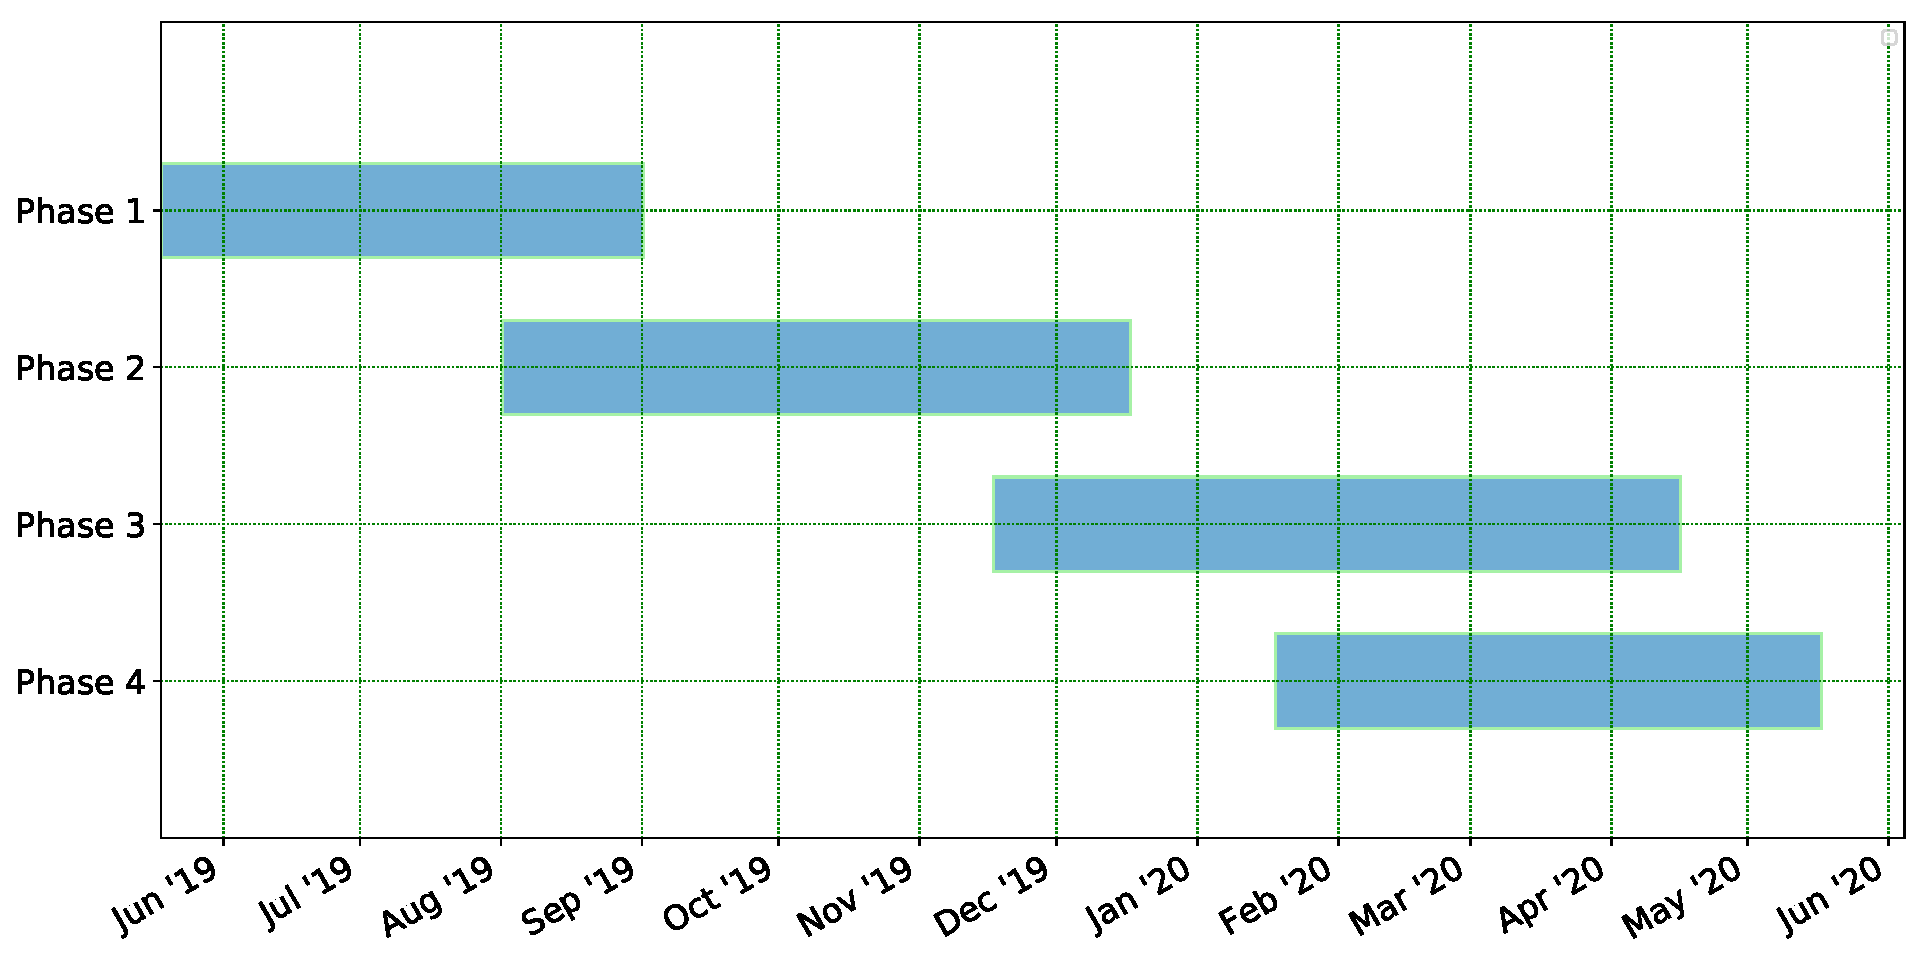
\includegraphics[width=.95\textwidth]{./phd_plan.pdf}
	\caption{Planned timeline of proposed research}\label{tab:work_plan}
\end{figure*}

\subsubsection{Phase 1: Design and implementation self-configuring property}

Month 1 would include design discussions for a prototype of the execution system. 
Result of these discussions will be the requirements of the middleware and its 
API. Design will be finalized and a prototypical implementation will be completed 
by Month 4. Capability to self-configure in terms of resources based on the desired 
workflow will mark the success of Phase 1.

\subsubsection{Phase 2: Implementation self-monitoring, self-regulating properties
and Continuous Integrated Testing}
Phase 2 includes defining the requirements for self-monitoring, and self-regulating 
properties and implement them in the middleware. End of phase 2 will include the 
\textit(self-*) properties as well as a Continuous integrated testing protocol to 
always verify the functionality of the middleware. Phase 2 spans from months 3 up 
to 6

\subsubsection{Phase 3: Integration with scientific workflows}
Phase 3 of the plan includes the integration of the proposed autonomic system with 
RADICAL-EnTK~\cite{balasubramanian2018harnessing} and start utilize the system for 
scientifc workflows in Satelite Imagery analysis and Molecular Dynamics simulation 
workflows. This phase spans between months 6 and 9.

\subsubsection{Phase 4: Investigation for an empirical model}

Experiments with synthetic and real applications with the prototype as well as 
scientific workflows will be used to investigate and derive empirical models. 
These models may be used to further generalize the behavior of the autonomic 
middleware based on application requirements. Phase 4 will overlap with Phase 2 
and 3 to utilize experiments done during those phases.

% ---------------------------------------------------------------------------
% Why
\subsection{Significance and impact of work}
Several scientific applications are required to be executed several times with 
different input data or initial conditions. The required concurrency to minimize 
the execution time of each run is not necessarily constant and may change based 
on the initial conditions. The autonomic management system suggested in this 
proposal will be the first to make resource configuration decisions for the users. 
This will lead to less time invested by users to make execution decisions about 
their workflows. These decisions will lead to better resource utilization and, 
as a result, better domain science. The empirical models derived by this work can 
be used to derive formal mathematical models.

% ---------------------------------------------------------------------------
% Challenges
\subsection{Challenges/Risks}

We estimate the proposed work, divided into four major phases, to take 12 months 
and we allocate 3 months to account for unforeseen circumstances. We would like 
to keep the committee aware of the following challenges that we see:

\begin{itemize}
	\item Design and Implementation (phases 1 \& 2) is iterative and special attention 
	needs to be given to the number of iterations against specific objectives, 
	given the timeline.
  \item All experiments performed on HPC systems are subject to variable queue 
	times and may limit the number of experiments performed in phase 2 and 4.
	\item Although the middleware will be well tested (80--90\% of the code base 
	will be covered by unit tests) and less susceptible to major changes, RADICAL-Pilot 
	is known to be less stable and is susceptible to changes as it serves multiple 
	projects. Stability of RADICAL-Pilot is considered in the estimates, but needs 
	to be made aware to the committee.
	\item Lastly, the HPC systems themselves may often become inaccessible due to 
	unplanned outages.
\end{itemize}

\bibliographystyle{plain}
\bibliography{proposal}
\end{document}\textit{}